\chapter{Bestimmung der Detektoreffizienz}
\section{Theoretische Grundlagen}
\subsection{Detektoreffizienz}
Die Wahrscheinlichkeit, dass ein $\gamma$-Photon mit der Energie $E$ im Detektor ein Photopeak-Signal erzeugt, wird mit der Detektoreffizienz $\epsilon(E_\gamma)$ beschrieben. Sie ist definiert als das
Verhältnis der tatsächlich registrierten Photopeak-Ereignisse $N_{\text{detektiert}}$
zur Anzahl der Gammaquanten, die den Detektor erreichen $N_{\text{erreicht}}$:
\begin{equation}
    \epsilon(E_\gamma)=\frac{N_{detektiert}}{N_{erreicht}}\approx\frac{N_{detektiert}}{B}\cdot\frac{4\pi D^2}{\pi d^2}, \text{wobei B die Aktivität der Probe ist}
\end{equation}
\label{eq_5}
Da die absolute Aktivität der Quelle $A$ bekannt ist, ergibt sich:
\begin{align*}
    N_{\text{erreicht}} = A \cdot P_\gamma \cdot t \cdot \frac{\Omega}{4\pi}
\end{align*}
wobei $P_\gamma$ die Übergangswahrscheinlichkeit der betrachteten Linie,
$t$ die Messdauer und $\Omega$ der vom Detektor überdeckte Raumwinkel ist.
Für kleine Winkel gilt näherungsweise:
\begin{align*}
    \frac{\Omega}{4\pi} \approx \frac{\pi d^2}{4\pi D^2} = \frac{d^2}{4D^2},
\end{align*}
wobei d der Detektordurchmesser und D der Abstand von der Quelle zum Detektor ist.
Daraus folgt für die Detektoreffizienz:
\begin{align*}
    \varepsilon(E_\gamma) \approx \frac{N_{\text{detektiert}}}{A \cdot P_\gamma \cdot t}\cdot \frac{4\pi D^2}{\pi d^2}.
\end{align*}
Die Effizienz nimmt mit steigender Energie ab, da hochenergetische Gammaquanten eine geringere Wahrscheinlichkeit besitzen, vollständig im Detektor absorbiert zu werden.

\section{Durchführung}
Zur Bestimmung der Effizienz des HPGe-Detektors wurden Spektren der $^{137}\mathrm{Cs}$- und $^{152}\mathrm{Eu}$-Quellen aufgenommen. Für jede Gamma-Linie wurde die Peakfläche durch Integration bestimmt und um den Untergrund korrigiert. Die Messdauer, der Abstand zwischen Quelle und Detektor sowie die geometrischen Parameter wurden konstant gehalten.
Aus den bekannten Aktivitäten der Quellen und den tabellierten Übergangswahrscheinlichkeiten der jeweiligen Gamma-Linien wurde die erwartete Anzahl der den Detektor erreichenden Gammaquanten berechnet. Durch Vergleich mit den gemessenen Photopeak-Ereignissen ergibt sich die Effizienz für jede Energie.

Die Schwellenwertfunktion \(B(\text{Cs})\) sowie der Abstand sind Tabelle \ref{tab_eff_1} zu entnehmen. Basierend auf der Detektionsrate \(N_\text{detect} = A\) (Tabellen \ref{taba_2} und \ref{taba_3}), die so bestimmten Effizienzen betragen für die $661keV$-Linie:
\begin{align*}
    \varepsilon_{\text{HPGe}}(661\,\mathrm{keV}) = (4,705 \pm0,042)\\
    \varepsilon_{\text{NaI}}(661\,\mathrm{keV}) = (11,269\pm0,461).
\end{align*}
Die Fehler ergeben sich aus den Unsicherheiten der Peakflächenbestimmung, der Aktivität sowie der geometrischen Parameter.

Die Ergebnisse zeigen, dass nur ein geringer Anteil der einfallenden 661-keV-Photonen im Photopeak erscheint. Die meißten Photonen durchlaufen den Detektor, werden gestreut oder erzeugen kein Signal im Photopeak, sei es aufgrund von Effekten während der Ladungssammlung (z. B. Rekombination) oder durch das Ausbleiben photoelektrischer Ereignisse im Photomultiplier (PMT).

Des Weiteren ist die Effizienz von Szintillationsdetektoren bei diesen Energien höher als die von Halbleiterdetektoren. Dieses Ergebnis entspricht den Erwartungen, da die höhere Ordnungszahl von Iod (\(Z = 53\)) im Vergleich zu Germanium (\(Z = 32\)) zu einem größeren Wirkungsquerschnitt für den photoelektrischen Effekt (\(\sigma_\text{photo} \propto Z^5\)) führt.

Analog zum Cäsium-Fall lassen sich die Effizienzen für das gesamte Europium-Spektrum bestimmen. Dabei ist zu beachten, dass die Referenzfunktion \(B(E)\) für jede Energie \(E\) mit der entsprechenden Zählrate verglichen werden muss (siehe Tabelle \ref{tab_eff_1}). Abbildung \ref{fig:eff_1} stellt die erzielten Ergebnisse in Form einer Effizienzkurve dar.

% add plots
\begin{figure}[H]
    \centering
    \begin{subfigure}[t]{0.48\textwidth}
        \centering
        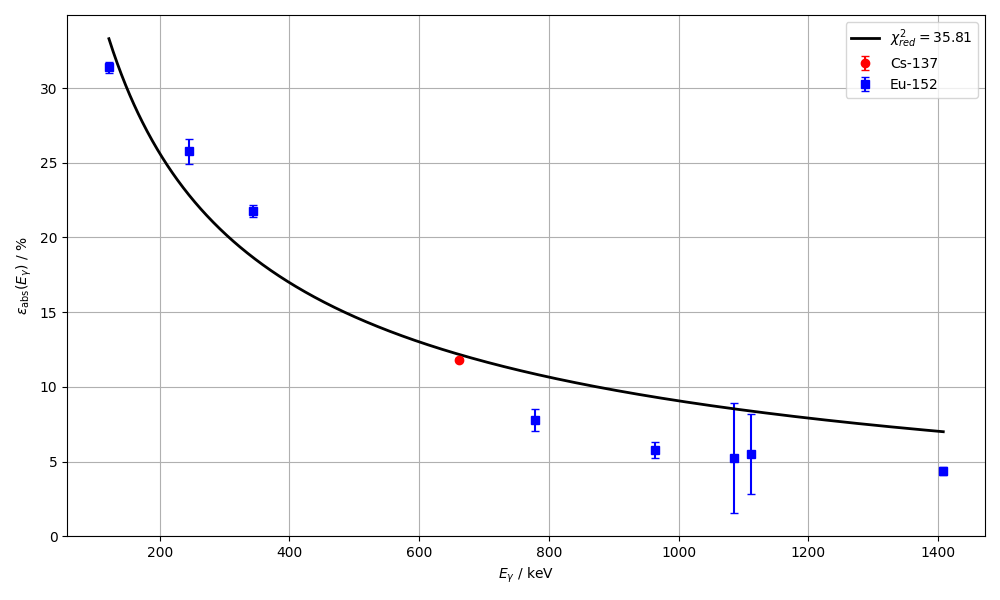
\includegraphics[width=\linewidth]{figs/Na_effizienz.png}
        \caption{NaI-Szintillationsdetektor}
        \label{fig:eff_1_1}
    \end{subfigure}
    \hfill
    \begin{subfigure}[t]{0.48\textwidth}
        \centering
        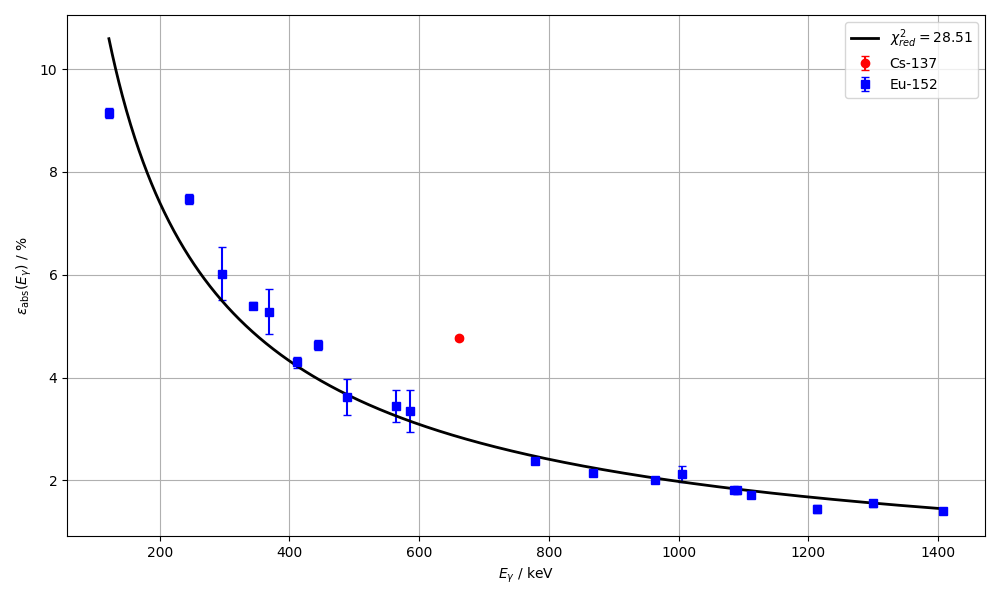
\includegraphics[width=\linewidth]{figs/Ge_effizienz.png}
        \caption{HPGe-Halbleiterdetektor}
        \label{fig:eff_1_2}
    \end{subfigure}
    
    \caption{Effizienz $\epsilon(E_\gamma)$ der Detektoren anhand des $^{152}$Eu-Spektrums}
    \label{fig:eff_1}
\end{figure}

Abbildung \ref{fig:eff_1} zeigt, dass die Effizienz \(\epsilon(E)\) beider Detektoren mit zunehmender Energie im Bereich \(E \in [90\,\text{keV}, 1400\,\text{keV}]\) deutlich abnimmt. Dieses Verhalten ist bekannt und lässt sich durch die folgende empirische Anpassungsfunktion beschreiben:\cite{Knoll1989_RadDet}

\[\epsilon(e) = \exp\!\left(-a_1\, e + a_2\, e^2\right),
\qquad e = \ln\!\left(\frac{E}{1.022\,\text{keV}}\right).
\tag{8}
\]

Die in den Abbildungen \ref{fig:eff_1_1} und \ref{fig:eff_1_2} dargestellten Effizienzkurven folgen dieser Funktionsform mit den folgenden Parametern:

für den HPGe-Detektor:

$a_1 = (0.242496 \pm 0.005806), \qquad a_2 = (-0.047522 \pm 0.000903)$\\


für den NaI(Tl)-Detektor:

$a_1 = (-0.039229 \pm 0.014094), \qquad a_2 = (-0.056339 \pm 0.002607)$

Die Anpassung beschreibt den Effizienzabfall bei höheren Energien gut. Allerdings gibt diese Anpassungsfunktion den erwarteten Effizienzverlauf bei sehr niedrigen Energien nicht präzise wieder. Insbesondere beim HPGe-Detektor (Abbildung \ref{fig:eff_1}) zeigen die Messpunkte im niederenergetischen Bereich keinen glockenförmigen Anstieg, sondern einen nahezu monotonen Abfall.

Trotz dieser Einschränkung liefert die Regression eine konsistente Beschreibung des Effizienzverhaltens im Energiebereich oberhalb von etwa $200keV$ und stimmt mit der aus der Cäsium-Messung bestimmten Effizienz bei $661keV$ überein. Sie liefert somit eine konsistente Darstellung der Detektoreffizienz in Abhängigkeit von der Energie im untersuchten Bereich.

\chapter{Aktivität $^{60}$Co}
Schließlich wird die Gültigkeit der berechneten Effizienzkurven überprüft, indem die Aktivität der Kobaltquelle aus dem gemessenen Spektrum rekonstruiert wird. Dazu werden zunächst die beiden Photopeaks bei $1173\,\mathrm{keV}$ und $1332\,\mathrm{keV}$ mittels Gauß-Fits ausgewertet. Die Effizienzfunktion basiert auf der Annahme, dass Ereignisse innerhalb des Fit-Bereichs vollständig absorbierte Gammaquanten repräsentieren. Daher werden die Peakflächen energieabhängig durch die Effizienz $\epsilon(E_\gamma)$ korrigiert.
Unter Verwendung der Parameter der Gauß-Funktionen wird zunächst ein „bereinigtes“ Kobalt-Spektrum erstellt, das keine linearen Untergrundkomponenten enthält:

\[
N'(K) =
\frac{A_1}{\sqrt{2\pi}\sigma_1}
\exp\!\left[-\frac{(K-\mu_1)^2}{2\sigma_1^2}\right]
+
\frac{A_2}{\sqrt{2\pi}\sigma_2}
\exp\!\left[-\frac{(K-\mu_2)^2}{2\sigma_2^2}\right].
\tag{9}
\]

Dieses bereinigte Spektrum wird anschließend kanalweise durch die Effizienz \(\epsilon(E(K))\) dividiert und über alle Kanäle aufsummiert. Dies ergibt die Anzahl der Photonen, die den Detektor während der Messdauer (T = 300 s) erreichen, bezeichnet als \(N_\text{reach}\).
\begin{align*}
    N_\text{reach} = \sum_i \frac{N'(K_i)}{\epsilon(E(K_i))}.
\end{align*}
Durch Division durch den Raumwinkel des Detektors und die Messdauer erhält man schließlich die Quellenaktivität \(B\):

\begin{equation}
    B = \frac{N_\text{reach}}{T} \frac{4\pi D^2}{\pi d^2}
    = \frac{4D^2}{d^2 T}\sum_i \frac{N'(K_i)}{\epsilon(E(K_i))}.   
\end{equation}

Die auf diese Weise berechneten Aktivitäten der Kobaltprobe betragen (Nennwert: \(B = 36.11\,\text{kBq}\) beim Vergleich mit Zerfallsgesetz):
\begin{align*}
    B_{\text{HPGe}} = (26.1 \pm 0.9)kBq,\\
    B_{\text{NaI}} = (8.5 \pm 0.6)kBq.
\end{align*}


Die berechneten Werte stimmen nicht mit der erwarteten Aktivität überein und bestätigen kaum die Gültigkeit der Effizienzkurven im Hochenergiebereich. Die relativ hohen Unsicherheiten sind vor allem auf die ungenaue Bestimmung der Abstände \(D\) und den daraus resultierenden Fehler durch den kleinsten Raumwinkel zurückzuführen. Auch die Übergangswahrscheinlichkeiten der
beiden $^{60}\mathrm{Co}$-Linien wurden nicht einbezogen, sodass die erwartete Photonenzahl fehlerhaft bestimmt wurde. Insgesamt ist die Rekonstruktion der Aktivität daher nur eingeschränkt aussagekräftig und bestätigt die Effizienzkurven im Hochenergiebereich nicht zuverlässig.